\chapter{Fundamentação Teórica}
Neste capítulo serão mostrados os conceitos matemáticos necessários para o entendimento desses objetivos.

%
% ARITMÉTICA MODULAR
%
\section{Aritmética Modular}
Na Teoria dos Números \cite{Niven:2014} (ramo da matemática pura que estuda os números inteiros), uma importante ferramenta é a aritmética modular,  a qual estuda as propriedades de conjuntos formados a partir dos restos da divisão de números inteiros por um inteiro \(n\), denominado módulo.

Dado qualquer inteiro positivo \(n\) e qualquer inteiro não negativo \(a\), se dividirmos \(a\) por \(n\), obteremos um quociente inteiro \(q\) e um resto inteiro \(r\), que obedecem ao seguinte relacionamento:
\begin{equation}
  a=qn+r \qquad 0 \leq r<n;\ q=\lfloor a/n \rfloor
\end{equation}

onde $\lfloor x \rfloor$ é o maior inteiro menor ou igual a \(x\).

Uma congruência é  uma relação entre dois números inteiros que, quando divididos por um mesmo número (chamado de módulo da congruência), deixam o mesmo resto.  Em termos formais, dois números inteiros \(a\) e \(b\) são congruentes módulo \(n\) se n divide a diferença \(a - b\).  Esta relação pode ser expressa por:

\begin{equation}
  a \equiv b \pmod n \label{eq:1}
\end{equation}

Para um inteiro positivo \(n\) e \(a\), \(b\), \(c\) inteiros quaisquer, a congruência tem as seguintes propriedades \cite{Stallings:2011}:
\begin{enumerate}
  \item $a \equiv b \pmod n$ se $n|(a - b)$.
  \item $a \equiv b \pmod n$ implica $b \equiv a \pmod n$.
  \item $a \equiv b \pmod n$ e $b \equiv c \pmod n$ implica $a \equiv c \pmod n$.
\end{enumerate}

Por definição, o operador $\pmod n$ mapeia todos os inteiros para o conjunto de inteiros $\{0, 1, ..., (n-1)\}$. Daí pode-se realizar operações aritméticas dentro dos limites desse conjunto, técnica conhecida como aritmética modular. A aritmética modular exibe as seguintes propriedades \cite{Stallings:2011}:
\begin{enumerate}
  \item $[a \pmod n + b \pmod n] \pmod n = (a + b) \pmod n$
  \item $[a \pmod n - b \pmod n] \pmod n = (a - b) \pmod n$
  \item $[a \pmod n \times b \pmod n] \pmod n = (a \times b) \pmod n$
\end{enumerate}

Em relação a divisão, ela não está definida em todos os casos. Se \(d\) é um inteiro que divide \(a\) e \(b\), então vale a relação apresentada na Equação \ref{eq:5}, onde \((n, d)\) é o maior divisor comum entre \(n\) e \(d\).

\begin{equation}
  \frac{a}{d} \equiv \frac{b}{d}\left(\mbox{mod}\ \frac{n}{(n,d)}\right) \label{eq:5}
\end{equation}

O inverso multiplicativo de a modulo \(n\), isto é, um inteiro \(b\) tal que \(a \times b = 1 \pmod  n\), existe apenas quando \((a, n) = 1\) (isto é, \(a\) e \(n\) são coprimos). O valor de \(b\) pode ser obtido através do Algoritmo de Euclides Estendido \cite{Halim:2013}.
\par A exponenciação modular calcula o resto de um número inteiro \(b\) quando elevado à um número inteiro \(k\) e é dividido por um inteiro positivo \(m\). Escolhidos a base \(b\), o expoente \(k\) e o módulo \(m\), uma exponenciação modular \(c\) é dada pela Equação \ref{eq:6}.

\begin{equation}
  c \equiv b^k\pmod m \label{eq:6}
\end{equation}

%
% ESTRUTURAS ALGÉBRICAS
%
\section{Estruturas Algébricas}

Antes de iniciar os estudos em aritmética de curvas elípticas, é importante
fixar alguns conceitos de álgebra. De acordo com Hefez,

\begin{citacao}
``Estruturas algébricas são modelos abstratos para tratar em bloco várias situações matemáticas concretas em que em determinados conjuntos são definidas operações com propriedades semelhantes.'' \cite{Hefez:2008} (p. 12)
\end{citacao}

%
% GRUPOS
%
\subsection{Grupos}

Um \textbf{grupo \((G,*)\)} é composto por um conjunto \(G\) e uma operação binária \(*\) sobre os elementos desse conjunto tal que os axiomas abaixo sejam satisfeitos \cite{Gilbert:2004}

\begin{enumerate}
\item O conjunto \(G\) é \textbf{fechado} para a operação \(*\)

$a * b \in G$ para todo $a,b \in G$.

\item A operação $*$ é \textbf{associativa}

$(a * b) * c = a * (b * c)$ para todo $a,b,c \in G$.

\item Existe um \textbf{elemento identidade} $e \in G$ tal que para todo elemento $a \in G, a * e = a$.
\item Existe um \textbf{elemento inverso} \(a'\) para todo elemento $a \in G$ tal que $a' * a = e$ (elemento identidade).
\end{enumerate}

Se a operação é \textbf{comutativa}, ou seja, se $a * b = b * a$ para todo $a, b \in G$, então o grupo é denominado \textbf{abeliano} (ou \textbf{comutativo}) em homenagem ao matemático Niels Abel. \cite{Gilbert:2004}

Exemplos de grupos abelianos são $(Z, +)$, $(R, +)$, ambos com identidade 0 e com infinitos elementos. ``O numero de elementos de um grupo é a sua \textbf{ordem}'' \cite{Coutinho:2014} (pg. 134). Para este trabalho, os grupos de maior interesse são aqueles que possuem ordem finita.

\subsection{Subgrupos}
Seja $(G, *)$ um grupo, e \(H\) um subconjunto não vazio de \(G\). Se $(H, *)$ satisfaz todos os axiomas de grupo, então diz-se que $(H, *)$ é um subgrupo de $(G, *)$\cite{Coutinho:2014}, ou seja

\begin{enumerate}
\item Para todo $a, b \in H$, $a * b \in H$.
\item O elemento neutro de \(G\) está em \(H\) e também é seu elemento neutro(a demonstração não será feita nesse trabalho).
\item Existe um inverso \(a'\) para todo $a \in H$.
\end{enumerate}

Todo grupo possui pelo menos dois subgrupos, como pode ser visto na citação abaixo.


\begin{citacao}
``Se \(e\) indica o elemento neutro de \(G\), então obviamente \(e\) é um subgrupo de \(G\). É imediato, também, que o próprio \(G\) é um subgrupo de si mesmo. Esses dois subgrupos, ou seja, \(e\) e \(G\), são chamados de \textbf{subgrupos triviais} de \(G\)''. \cite{Domingues:2003} (pg. 154)
\end{citacao}

\subsection{Teorema de Lagrange}

Um teorema de grande importância para o estudo da criptografia é o teorema de Lagrange, este estabelece que, se $G$ é um grupo finito, e $H$ é um subgrupo de $G$, então a ordem de $H$ sempre divide a ordem de $G$ \cite{Shoup:2005}.A demostração deste teorema não será abordada nesse trabalho, mas seu resultado será de grande utilidade mais à frente, no estudo da criptografia de curvas elípticas.

\subsection{Homomorfismos de grupos}

Sejam os grupos $(G, \cdot)$ e $(H, \cdot)$, uma função $f: G \rightarrow H$ é chamada de \textit{homomorfismo} se $f(a \cdot b) = f(a) \cdot f(b)$ onde $a, b \in G$. Se a operação dos grupos for diferente, por exemplo, $(G, \cdot)$ e $(H, \star)$, então a condição é dada por $f(a \cdot b) = f(a) \star f(b)$ \cite{Gilbert:2004}.



%
% CORPOS FINITOS
%
\subsection{Corpos Finitos}



%
% CRIPTOGRAFIA
%
\section{Criptografia} \label{sec:criptografia}
Criptografia é a ciência que trata de cifrar a escrita, de modo a torná-la ininteligível para os que não tenham os métodos convencionados para ter acesso a ela. Em Tecnologia da Informação, esta definição é ampliada a fim de englobar não só a escrita, mas qualquer tipo de documento ou dados que devam ser tratados secretamente. Um Sistema de Criptografia define um sistema em que um texto (ou documento, ou qualquer tipo de dado) é transformado através da criptografia em um texto cifrado (\textit{ciphertext}) ou o texto cifrado é transformado de volta à informação original, através de algoritmos. A primeira ação é denominada cifragem ou criptografar, e a segunda é chamada de decifração ou decriptação. \cite{Portnoi:2005}

Com a criptografia pretende-se garantir que uma mensagem só será lida e compreendida pelo destinatário autorizado, e para isso, é necessário que se cumpram quatro requisitos:

\begin{itemize}
\item \textit{confidencialidade}: obtida pela encriptação dos dados, assegura que só os receptores autorizados terão acesso às informações da mensagem.
\item \textit{integridade}: assegura que a informação não será alterada durante o processo de transporte da informação. É obtida por meio da assinatura digital.
\item \textit{autenticação}: o remetente e o receptor podem confirmar as identidades uns dos outros assim como a origem e o destino da informação. É obtida por meio da assinatura digital e dos certificados.
\item \textit{irretratabilidade}: ou não-repúdio é obtida por meio da assinatura digital e certificados, o remetente pode assiná-lo de forma digital, limitando legalmente a responsabilidade.
\end{itemize}

%
% CRIPTOGRAFIA SIMÉTRICA
%
\subsection{Criptografia simétrica}
A criptografia simétrica foi o primeiro tipo de criptografia criado. Funciona transformando um texto em uma mensagem cifrada, por meio da definição de uma chave secreta, que será utilizada posteriormente para decriptar a mensagem, tornando novamente um texto simples. \cite{Cavalcante:2015}

A criptografia simétrica utiliza apenas uma chave para codificar e decodificar uma mensagem. É usada em transmissões de dados em que não é necessário um grande nível de segurança como mensagens enviadas de um computador para outro, nas comunicações entre duas máquinas, no armazenamento da informação em um disco rígido.

A criptografia simétrica é relativamente rápida, contudo como desvantagem, não só o transmissor deve conhecer a chave como também o receptor. Além disso, o volume total dos dados transmitidos é limitado pelo tamanho da chave.

%
% CRIPTOGRAFIA ASSIMÉTRICA
%
\subsection{Criptografia assimétrica}
Utiliza duas chaves, uma para criptografar os dados (chamada de chave pública) e outra para decifrar os dados (chamada de chave privada). Neste caso a chave pública é divulgada enquanto que a chave privada permanece secreta. Esta técnica é muito utilizada para o envio de mensagens onde se deseja que somente o destinatário, portador da chave privada, consiga ler a mensagem. O emissor da mensagem utiliza a chave pública para criptografar a mensagem e a envia, quando o receptor receber a mensagem utilizará a chave privada para decifrar a mensagem. Este esquema provê a confidencialidade dos dados e também autenticação pois somente o proprietário da chave privada será capaz de decifrar a mensagem. Nestes algoritmos um dado que é criptografado com uma chave só poderá ser decifrado com a utilização da outra chave e vice-versa.

%
% CURVAS ELÍPTICAS
%
\section{Curvas Elípticas}

\subsection{Definição}
Curvas elípticas não são elipses. Elas têm esse porque são descritas por equações cúbicas, semelhantes às usadas para calcular a circunferência de uma elipse. Em geral, as equações cúbicas para curvas elípticas têm a forma
\begin{equation}
y^2 + axy + by = x^3 + cx^2 + dx + e \label{eq:5}
\end{equation}
onde \(a, b, c, d\) e \(e\) são números reais e \(x\) e \(y\) assumem valores nos números reais. Equações deste tipo são chamadas de \textit{equações de Weiestrass}. Para a nossa finalidade, é suficiente limitarmos na forma normal da equação de Weiestrass
\begin{equation}
y^2 = x^3 + ax + b \label{eq:6}
\end{equation}

Essas equações são consideradas cúbicas, ou de grau 3, pois o expoente mais alto que elas contém é um 3. Também incluído na definição de uma curva elíptica está um único elemento indicado por \(O\) e chamado de \textit{ponto no infinito} ou \textit{ponto zero}.

A Figura \ref{fig:curvas} apresenta alguns exemplos de curvas elípticas usando a forma normal da equação de Weierestrass.

\begin{figure}[h]
\centering
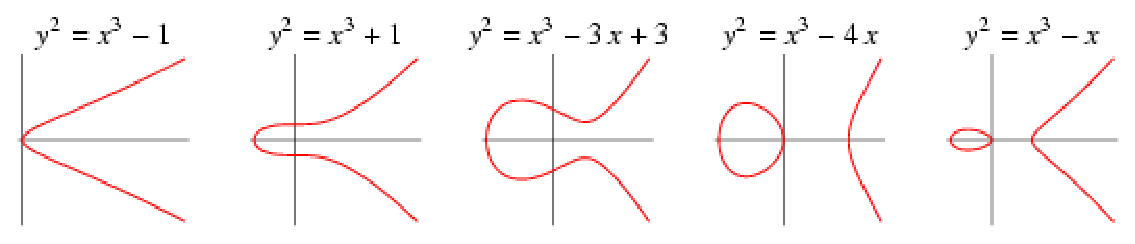
\includegraphics[scale=0.5, bb=0 0 529 101]{figuras/curvas.eps}
\caption{Exemplos de curvas elípticas}
\label{fig:curvas}
\end{figure}

Podemos mostrar que um grupo pode ser definido com base no conjunto E(\(a, b\)) para valores específicos de \(a\) e \(b\) na Equação \ref{eq:6}, desde que a condição a seguir seja atendida:
\begin{equation}
4a^3 + 27b^2 \neq 0 \label{eq:7}
\end{equation}

\subsection{Propriedades}
Uma importante característica da curvas elípticas é que existe uma forma natural de ``somar'' dois pontos produzindo um terceiro ponto. Para tanto, deve-se satisfazer a Equação \ref{eq:7}. No entanto, esta ``soma'' se refere à operação que combina dois pontos de maneira análoga da soma algébrica em alguns aspectos (é comutativa, associativa e existe um elemento identidade), mas bem diferente em outras formas.

Em termos geométricos, as regras para a adição podem ser indicadas da seguinte maneira: se três pontos em uma curva elíptica se encontram em uma linha reta, sua soma é \(O\). Por essa definição, podemos definir as regras da adição sobre uma curva elíptica:

\begin{figure}[h]
\centering
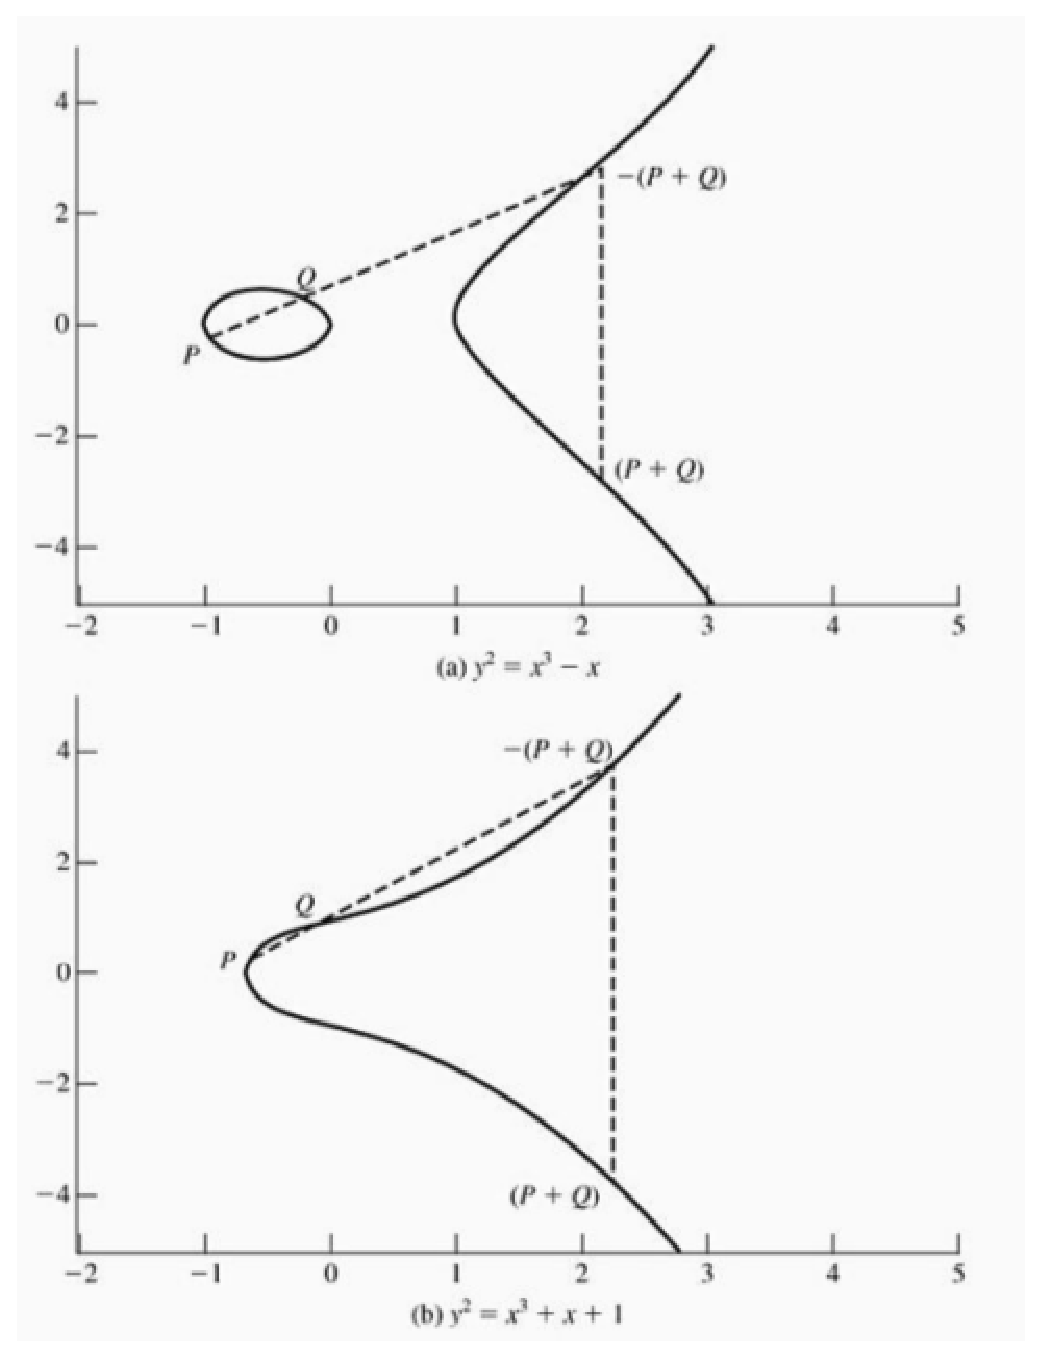
\includegraphics[scale=0.5, bb=0 0 484 636]{figuras/pontos_curva.eps}
\caption{Exemplos de soma de pontos em curvas elípticas}
\label{fig:pontos}
\end{figure}

\begin{enumerate}
  \item $O$ funciona como a identidade aditiva. Assim, $O = -O$; para qualquer ponto $P$ na curva elíptica, $P + O = P$. A seguir, consideramos $P \neq O$ e $Q \neq O$.
  \item O negativo de um ponto \(P\) é o ponto com a mesma coordenada \(x\), sem o negativo da coordenada \(y\); ou seja, se $P = (x, y)$, então $-P = (x, -y)$. Observe que esses dois pontos podem ser juntados por uma linha vertical. Observe que $P + (-P) = P - P = O$.
  \item Para somar dois pontos \(P\) e \(Q\) com coordenadas \(x\) diferentes, desenhe uma linha reta entre eles e encontre o terceiro ponto de interseção \(R\). Pode-se ver facilmente que existe um único ponto \(R\) que é o ponto de interseção (a menos que a linha seja tangente à curva em \(P\) ou \(Q\), quanto consideramos $R=P$ ou $R=Q$, respectivamente). Para formar uma estrutura de grupo, precisamos definir a adição sobre três pontos da seguinte forma: $P+Q=-R$. Ou seja, definimos $P+Q$ como sendo a imagem-espelho (com relação ao eixo \(x\)) do terceiro ponto da interseção. A figura \ref{fig:pontos}
  \item A interpretação geométrica do item anterior também se aplica a dois pontos, \(P\) e \(-P\), com a mesma coordenada \(x\). Os pontos são reunidos por uma linha vertical, que também pode ser vista como a interseção da curva no ponto infinito. Portanto, temos $P+(-P)=O$, coerente com o item (2).
  \item Para dobrar um ponto \(Q\), desenhe uma linha tangente e encontre o outro ponto da interseção \(S\). Então, $Q+Q=2Q=-S$.
\end{enumerate}

Com a lista de regras apresentada, pode-se se mostrar que o conjunto E(\(a, b\)) é um grupo abeliano. \cite{Stallings:2011}

\subsection{Curvas elípticas sobre corpo finito}
A criptografia de curva elíptica utiliza curvas elípticas em que as variáveis e coeficientes são todos restritos a elementos de um corpo finito, ou seja, assumem valores no conjunto de inteiros de 0 até $p - 1$ em que os cálculos são realizados módulo \(p\). Desta forma, é dito que a curva está sobre $\mathbb{F}_p$. \cite{Stallings:2011}

\begin{equation}
y^2 \mod p = (x^3 + ax + b) \mod p
\end{equation}

Pode-se mostrar que um grupo abeliano finito é definido com base no conjunto $E_p(a, b)$, desde que $(x^3 + ax + b) \mod p$ não tenha fatores repetidos. Isso é equivalente à condição

\begin{equation}
(4a^3 + 27b^2) \mod p \neq 0 \label{eq:13}
\end{equation}

A Equação \ref{eq:13} tem a mesma forma da Equação \ref{eq:7}. As regras para adição sobre $E_p(a, b)$ correspondem à técnica algébrica descrita para as curvas elípticas definidas sobre números reais. Para todos os pontos $P, Q \in E_p(a, b)$.

\begin{figure}[h]
\centering
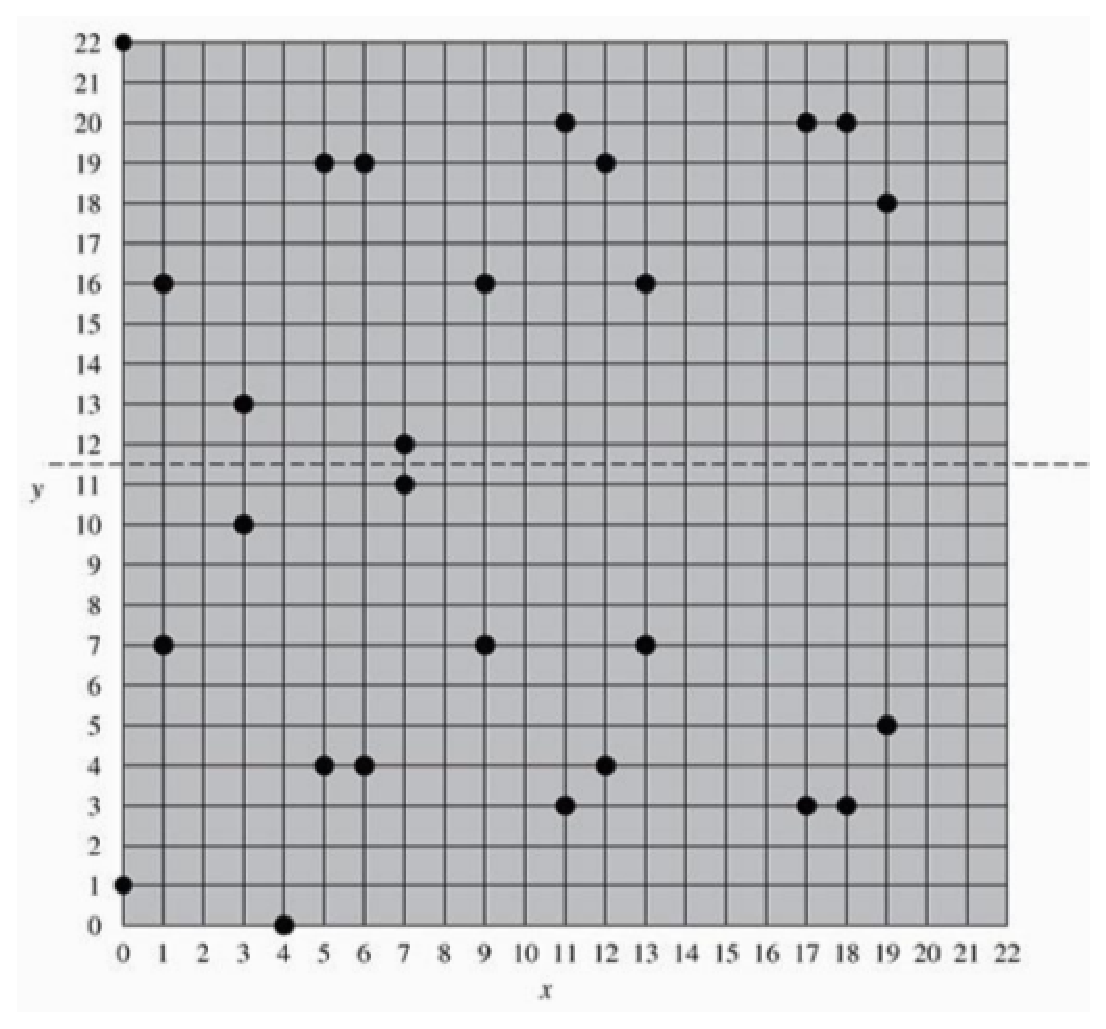
\includegraphics[scale=0.6, bb=0 0 515 478]{figuras/curva_sobre_corpo_finito.eps}
\caption{Curva elíptica $E_{23}(1, 1)$}
\label{fig:curvas}
\end{figure}

\begin{enumerate}
  \item $P + O = P$.
  \item Se $P = (x_P, y_P)$, então $P + (x_P, -y_P) = O$. O ponto $(x_P, -y_P)$ é o negativo de \(P\), indicado como \(-P\).
  \item Se $P = (x_P, y_P)$ e $Q = (x_Q, y_Q)$ com $P \neq -Q$, então $R = P + Q = (x_R, y_R)$ é determinado pelas seguintes regras:
    \begin{eqnarray*}
    x_R &=& (\lambda^2 - x_P - x_Q) \mod p \\
    y_R &=& (\lambda(x_P - x_R) - y_P) \mod p
    \end{eqnarray*}
  onde
    \begin{eqnarray*}
    \lambda =
    \begin{cases}
    \left(\dfrac{y_Q - y_P}{x_Q - x_P}\right) \mod p \textrm{, se} \ P \neq Q \\ \\
    \left(\dfrac{3x_P^2 + a}{2y_P}\right) \mod p \textrm{, se} \ P = Q
    \end{cases}
    \end{eqnarray*}
  \item A multiplicação é definida como adição repetida; por exemplo, $4P = P + P + P + P$.
\end{enumerate}

%
% ECDPL
%
\subsection{O problema do logaritmo discreto sobre curvas elípticas} \label{ecdpl}
Seja \(E\) uma curva elíptica sobre o corpo finito $\mathbb{F}_p$ e seja \(P\) e \(Q\) pontos em $E_p(a, b)$. O problema do logaritmo discreto sobre curvas elípticas ECDLP (\textit{Elliptic Curve Discrete Logarithm Problem}) é o problema de encontrar um inteiro \(n\) tal que $Q = nP$. Pela analogia com o problema do logaritmo para $\mathbb{F}_p^*$, denotamos esse inteiro \(n\) por

\begin{eqnarray*}
nP &=& Q \\
n &=& \log_P(Q)
\end{eqnarray*}

e chamamos \(n\) como logaritmo discreto elíptico de \(Q\) em relação a \(P\). \cite{Hoffstein:2008}

%
% CRIPTOGRAFIA DE CURVAS ELÍPTICAS
%
\subsection{Criptografia de curvas elípticas}
Primeiro, selecione um inteiro grande \(p\) que seja primo e parâmetros da curva elíptica \(a\) e \(b\) de acordo com a equação \ref{eq:5} ou \ref{eq:6}. Isso define o grupo elíptico de pontos $E_q(a, b)$. Em seguida escolha um ponto base $G = (x_1, y_1)$ em $E_q(a, b)$, cuja a ordem seja um valor muito grande \(n\). $E_q(a, b)$ e \(G\) são os parâmetros do criptossistema, conhecidos por todos os participantes.

Um acordo de chaves entre os usuários A e B pode ser realizado da seguinte maneira:
\begin{enumerate}
\item \textbf{A} seleciona um inteiro \(n_A\) menor que \(n\). Essa é chave privada de \textbf{A}, então \textbf{A} gera sua chave pública $P_A = n_A \times G$
\item Do mesmo modo, \textbf{B} seleciona um inteiro \(n_B\) menor que \(n\), sendo essa a chave privada de \textbf{B}. E então \textbf{B} calcula e divulga sua chave pública $P_B = n_B \times G$.
\item \textbf{A} gera a chave secreta $k = n_A \times P_B$. \textbf{B} gera a chave secreta $k = n_B \times P_A$
\end{enumerate}

Os dois cálculos na etapa 3 produzem o mesmo resultado, porque
\begin{equation*}
n_A \times P_B = n_A \times (n_B \times G) = n_B \times (n_A \times G) = n_B \times P_A
\end{equation*}

Para quebrar esse esquema, um atacante teria de ser capaz de calcular \(k\) a partir de \(kG\), o que é considerado difícil. Este problema que é conhecido como problema do \textit{\textbf{logaritmo discreto sobre curvas elípticas}}, como já explicado em \ref{ecdpl}.

